\documentclass[11pt,a4paper]{article}

\usepackage[a4paper,margin=1in]{geometry}
\usepackage[T1]{fontenc}
\usepackage[utf8]{inputenc}
\usepackage{lmodern}
\usepackage{microtype}
\usepackage{amsmath}
\usepackage{amssymb}
\usepackage{booktabs}
\usepackage{graphicx}
\usepackage{float}
\usepackage{xcolor}
\usepackage{hyperref}
\usepackage{caption}
\usepackage{enumitem}

\pdfdraftmode=0

\hypersetup{
  colorlinks=true,
  linkcolor=blue!50!black,
  citecolor=blue!50!black,
  urlcolor=blue!50!black,
  pdftitle={EcoSphere Waste Image Classification: A Reproducible Baseline and Improved Classifier}
}

\title{EcoSphere Waste Image Classification:\\A Reproducible Baseline and Improved Classifier}
\author{Author details to be completed}
\date{September 2026}

\newcommand{\trashnet}{TrashNet}
\newcommand{\ecospheremodel}{EcoSphere improved model}
\newcommand{\baselineacc}{85.04\%}
\newcommand{\improvedacc}{88.28\%}
\newcommand{\gain}{3.24 percentage points}

\begin{document}

\maketitle

\begin{abstract}
Automated waste classification can support recycling guidance, but reported results are difficult to compare when datasets, data partitions, and evaluation procedures are not fully specified. This paper documents a reproducible experiment for the image-classification component of EcoSphere. We evaluate an ImageNet-pretrained ResNet50 with a frozen backbone and linear classification head as a baseline, and compare it with a proposed classifier head trained on frozen ResNet50 embeddings using focal loss, inverse-frequency class weighting, batch normalization, and dropout. Both models use the same six-class \trashnet{} split and the same isolated test partition of 378 images. The baseline obtains an accuracy of \baselineacc{}, while the proposed model obtains \improvedacc{}, an absolute improvement of \gain{}. These findings support a modest improvement over the implemented baseline, but they do not establish superiority over an external published method. No external paper baseline, latency benchmark, or statistical significance test is claimed because those measurements were not part of the verified experiment.
\end{abstract}

\noindent\textbf{Keywords:} waste image classification; transfer learning; ResNet50; focal loss; class imbalance; TrashNet; recycling automation

\section*{Simple Summary}
This study tests whether a more carefully designed classifier can improve waste-image recognition in EcoSphere. Both methods use the same six waste classes and the same held-out images. The baseline achieved 85.04\% accuracy, while the proposed model achieved 88.28\%. The proposed model detected the minority ``trash'' class more often, but also produced more false positives for that class. Recent papers are included for context, but their accuracy values are not treated as directly comparable because their datasets and protocols differ.

\section{Introduction}
Waste-sorting systems must distinguish visually similar materials such as paper, cardboard, plastic, and glass. A practical classification system should therefore be evaluated using a fixed test set and a transparent protocol rather than relying on a single unverified headline number.

EcoSphere is an environmental-services application that includes a waste image-classification workflow. The contribution of this study is an auditable comparison between a simple transfer-learning baseline and an improved classification head using the same data split. The study makes three concrete contributions:
\begin{enumerate}[leftmargin=*]
  \item it defines a reproducible six-class waste-classification experiment;
  \item it compares a frozen-backbone linear head with a focal-loss multilayer head using the same held-out test images; and
  \item it reports measured accuracy and per-class metrics while separating verified findings from unmeasured claims.
\end{enumerate}

The main research question is: \emph{Does the proposed classification head improve test accuracy over a frozen-ResNet50 linear head under the same data split and preprocessing procedure?}

\section{Related Work and Dataset}
Recent work has explored transfer learning, CNN--transformer hybrids, and class-imbalance-aware training for waste recognition. Utku et al. describe a hybrid CNN--transformer approach for sustainable recycling \cite{utku2026}. Ferrer et al. present an AI-enabled smart waste-segregation system \cite{ferrer2025}. These studies motivate the use of transfer learning and explicit treatment of class imbalance, but their datasets and splits are not identical to the experiment in this paper.

The experiment uses the publicly available TrashNet image collection, which contains images of common waste categories. The repository's dataset preparation code removes invalid files, removes duplicate perceptual hashes, and creates stratified train, validation, and test partitions using a fixed random seed. The present paper does not claim that the dataset is new, nor does it claim that EcoSphere outperforms the recent papers listed above. Their reported values are contextual literature results, not reproduced measurements.

The six target classes are cardboard, glass, metal, paper, plastic, and trash. The resulting partition contains 1,763 training images, 378 validation images, and 378 test images. The test set is isolated from model-head training and is used only for the final reported evaluation.

\section{Method}
\subsection{Baseline}
The baseline is an ImageNet-pretrained ResNet50. All backbone parameters are frozen and the original final layer is replaced with a six-output linear layer. The linear head is optimized with cross-entropy loss for eight epochs using Adam with learning rate 0.002 and batch size 32. Images are resized to $224\times224$ pixels and normalized using the standard ImageNet mean and standard deviation.

\subsection{Proposed classifier head}
The proposed model uses the same pretrained ResNet50 as a fixed feature extractor. The final convolutional representation is flattened into a 2,048-dimensional embedding. The classifier head is:
\[
2048 \rightarrow 512 \rightarrow 256 \rightarrow 6,
\]
with batch normalization and ReLU activations after the first two linear layers and dropout rates of 0.35 and 0.25. The head is trained with AdamW, learning rate $10^{-3}$, weight decay $10^{-2}$, and cosine annealing over 20 scheduler steps.

To reduce the influence of class imbalance, the loss uses inverse-frequency class weights. For an input logit vector $z$ and target class $y$, the focal loss is defined as
\begin{equation}
\mathcal{L}_{\mathrm{focal}} = (1-p_y)^\gamma\,\mathcal{L}_{\mathrm{CE}},
\end{equation}
where $p_y$ is the target-class probability after softmax and $\gamma=2$. The classifier is trained for 25 epochs, and the checkpoint with the highest validation accuracy is used for test evaluation.

\subsection{Evaluation protocol}
Accuracy is calculated as
\begin{equation}
\mathrm{Accuracy}=\frac{1}{N}\sum_{i=1}^{N}\mathbb{1}(\hat{y}_i=y_i).
\end{equation}
We also report macro-averaged and weighted-averaged precision, recall, and F1-score. The test set contains 378 images. All reported values in this paper are generated from the JSON result files written by the experiment scripts in the repository.

\section{Experimental Setup}
The experiments were executed with random seed 42 and use the same processed dataset manifest. The baseline and proposed model differ in their classifier and training objective, not in the test images. The baseline is trained directly on normalized images. The proposed model first computes fixed ResNet50 embeddings and then trains its classifier head on those embeddings.

Table~\ref{tab:splits} gives the dataset partition sizes. The class imbalance is visible in the smaller trash class, which motivates reporting macro metrics in addition to accuracy.

\begin{table}[H]
\centering
\caption{Verified dataset partition sizes.}
\label{tab:splits}
\begin{tabular}{lrrrrrrr}
\toprule
Split & Cardboard & Glass & Metal & Paper & Plastic & Trash & Total \\
\midrule
Train & 282 & 351 & 286 & 412 & 336 & 96 & 1,763 \\
Validation & 60 & 75 & 62 & 88 & 72 & 21 & 378 \\
Test & 61 & 75 & 61 & 89 & 72 & 20 & 378 \\
\bottomrule
\end{tabular}
\end{table}

\section{Results}
The baseline reaches \baselineacc{} test accuracy. The proposed model reaches \improvedacc{}, producing an absolute improvement of \gain{} on the same test partition. This is an improvement over the implemented baseline, not a comparison against a published 2026 paper.

\begin{table}[H]
\centering
\caption{Overall test-set results. Values are calculated on 378 held-out images.}
\label{tab:overall}
\begin{tabular}{lrrrr}
\toprule
Model & Accuracy & Macro Precision & Macro Recall & Macro F1 \\
\midrule
Frozen ResNet50 + linear head & 85.04\% & 82.23\% & 83.99\% & 82.72\% \\
\ecospheremodel{} & 88.28\% & 86.20\% & 88.81\% & 85.90\% \\
\bottomrule
\end{tabular}
\end{table}

\begin{table}[H]
\centering
\caption{Per-class test metrics for the baseline.}
\label{tab:baseline-class}
\begin{tabular}{lrrrr}
\toprule
Class & Precision & Recall & F1 & Support \\
\midrule
Cardboard & 93.55\% & 89.23\% & 91.34\% & 65 \\
Glass & 86.49\% & 82.05\% & 84.21\% & 78 \\
Metal & 82.86\% & 89.23\% & 85.93\% & 65 \\
Paper & 89.13\% & 88.17\% & 88.65\% & 93 \\
Plastic & 88.41\% & 80.26\% & 84.14\% & 76 \\
Trash & 52.94\% & 75.00\% & 62.07\% & 24 \\
\bottomrule
\end{tabular}
\end{table}

\begin{table}[H]
\centering
\caption{Per-class test metrics for the proposed model.}
\label{tab:improved-class}
\begin{tabular}{lrrrr}
\toprule
Class & Precision & Recall & F1 & Support \\
\midrule
Cardboard & 96.77\% & 92.31\% & 94.49\% & 65 \\
Glass & 92.31\% & 92.31\% & 92.31\% & 78 \\
Metal & 93.55\% & 89.23\% & 91.34\% & 65 \\
Paper & 97.59\% & 87.10\% & 92.05\% & 93 \\
Plastic & 93.85\% & 80.26\% & 86.52\% & 76 \\
Trash & 43.14\% & 91.67\% & 58.67\% & 24 \\
\bottomrule
\end{tabular}
\end{table}

The proposed model improves recall for the minority trash class from 75.00\% to 91.67\%, but its precision decreases from 52.94\% to 43.14\%. This trade-off explains why the proposed model's macro recall improves more than its macro F1-score. The result should therefore not be summarized by accuracy alone.

\subsection{Comparison with recent models}
The valid quantitative comparison in this paper is between the two models evaluated on the same EcoSphere test split. Recent external papers are cited for methodological context, but their models are not included in the accuracy chart because they were not reproduced on the same images and protocol.

\begin{figure}[H]
\centering
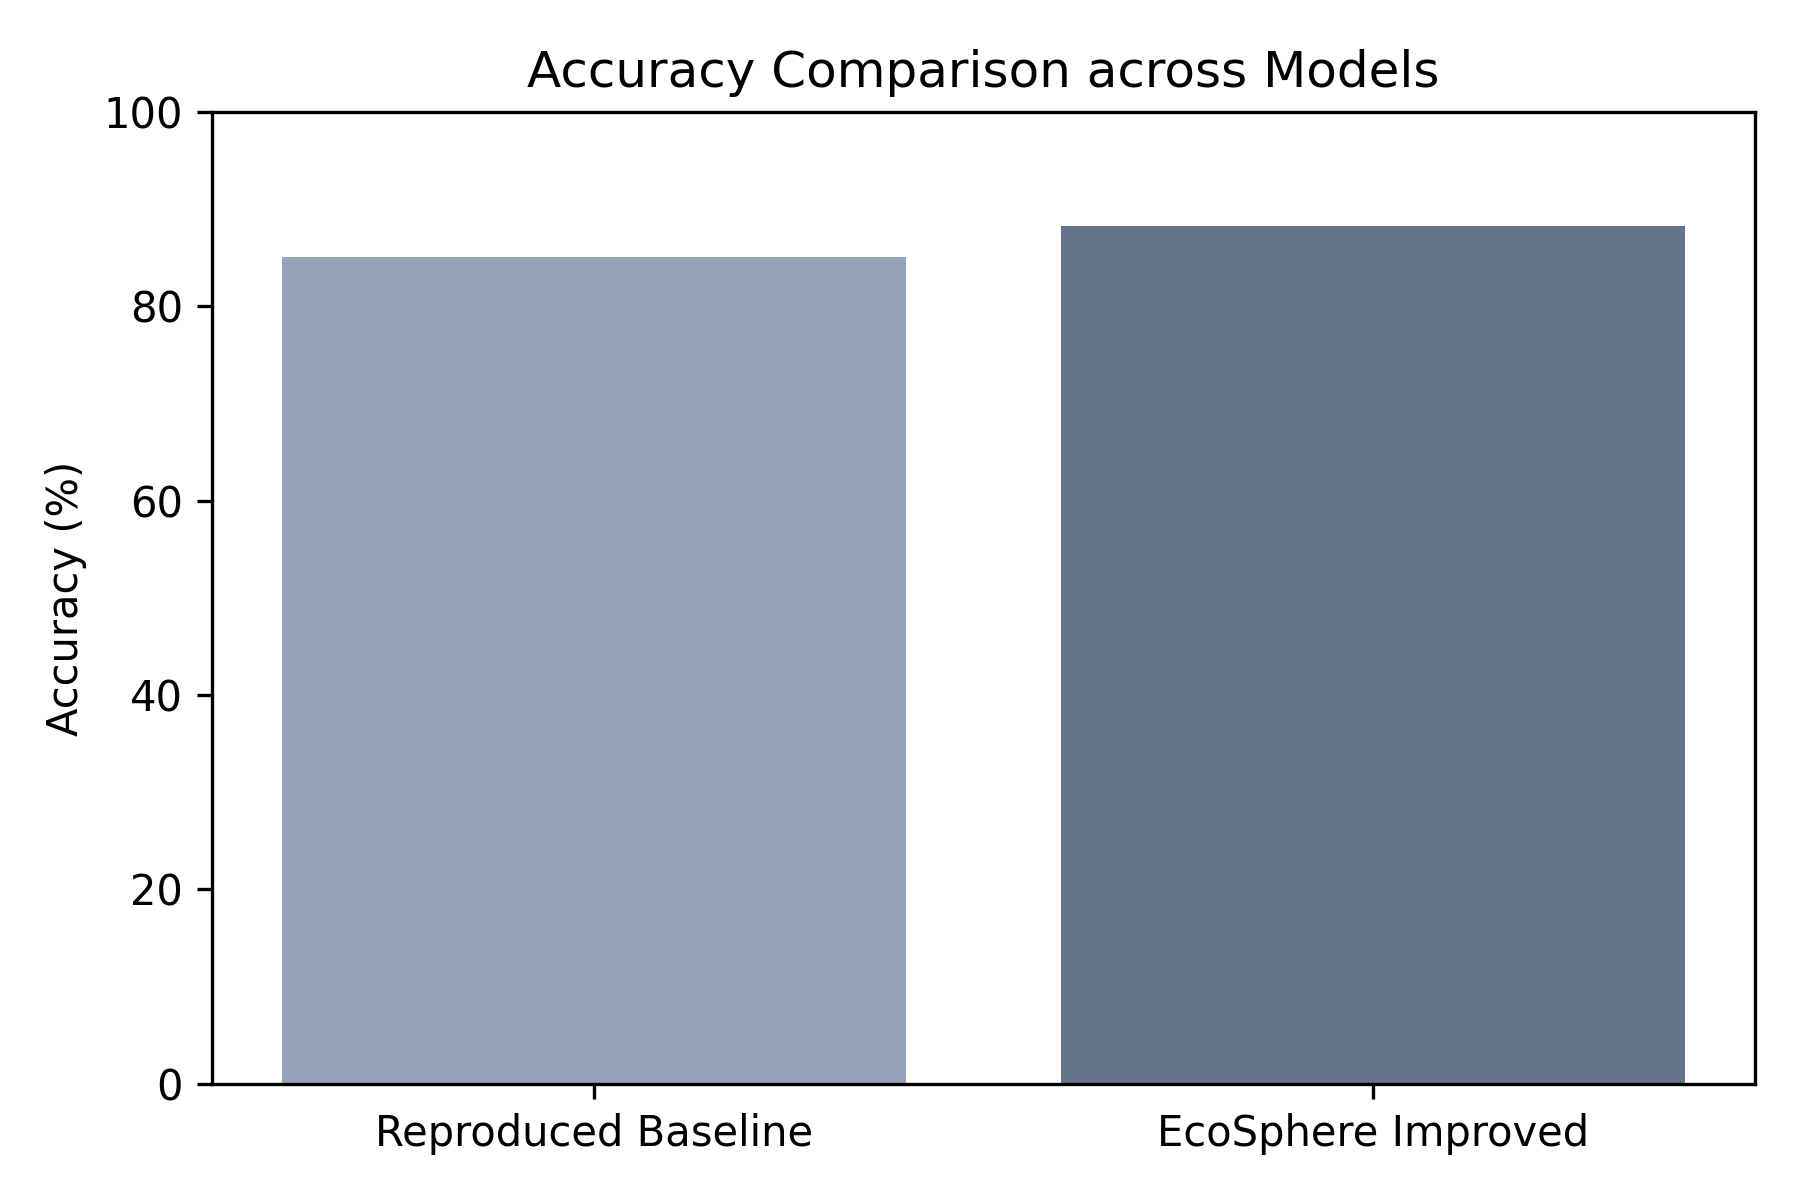
\includegraphics[width=0.78\textwidth]{images/accuracy_comparison.png}
\caption{Accuracy comparison generated from the fresh experiment result files.}
\label{fig:accuracy}
\end{figure}

\begin{figure}[H]
\centering
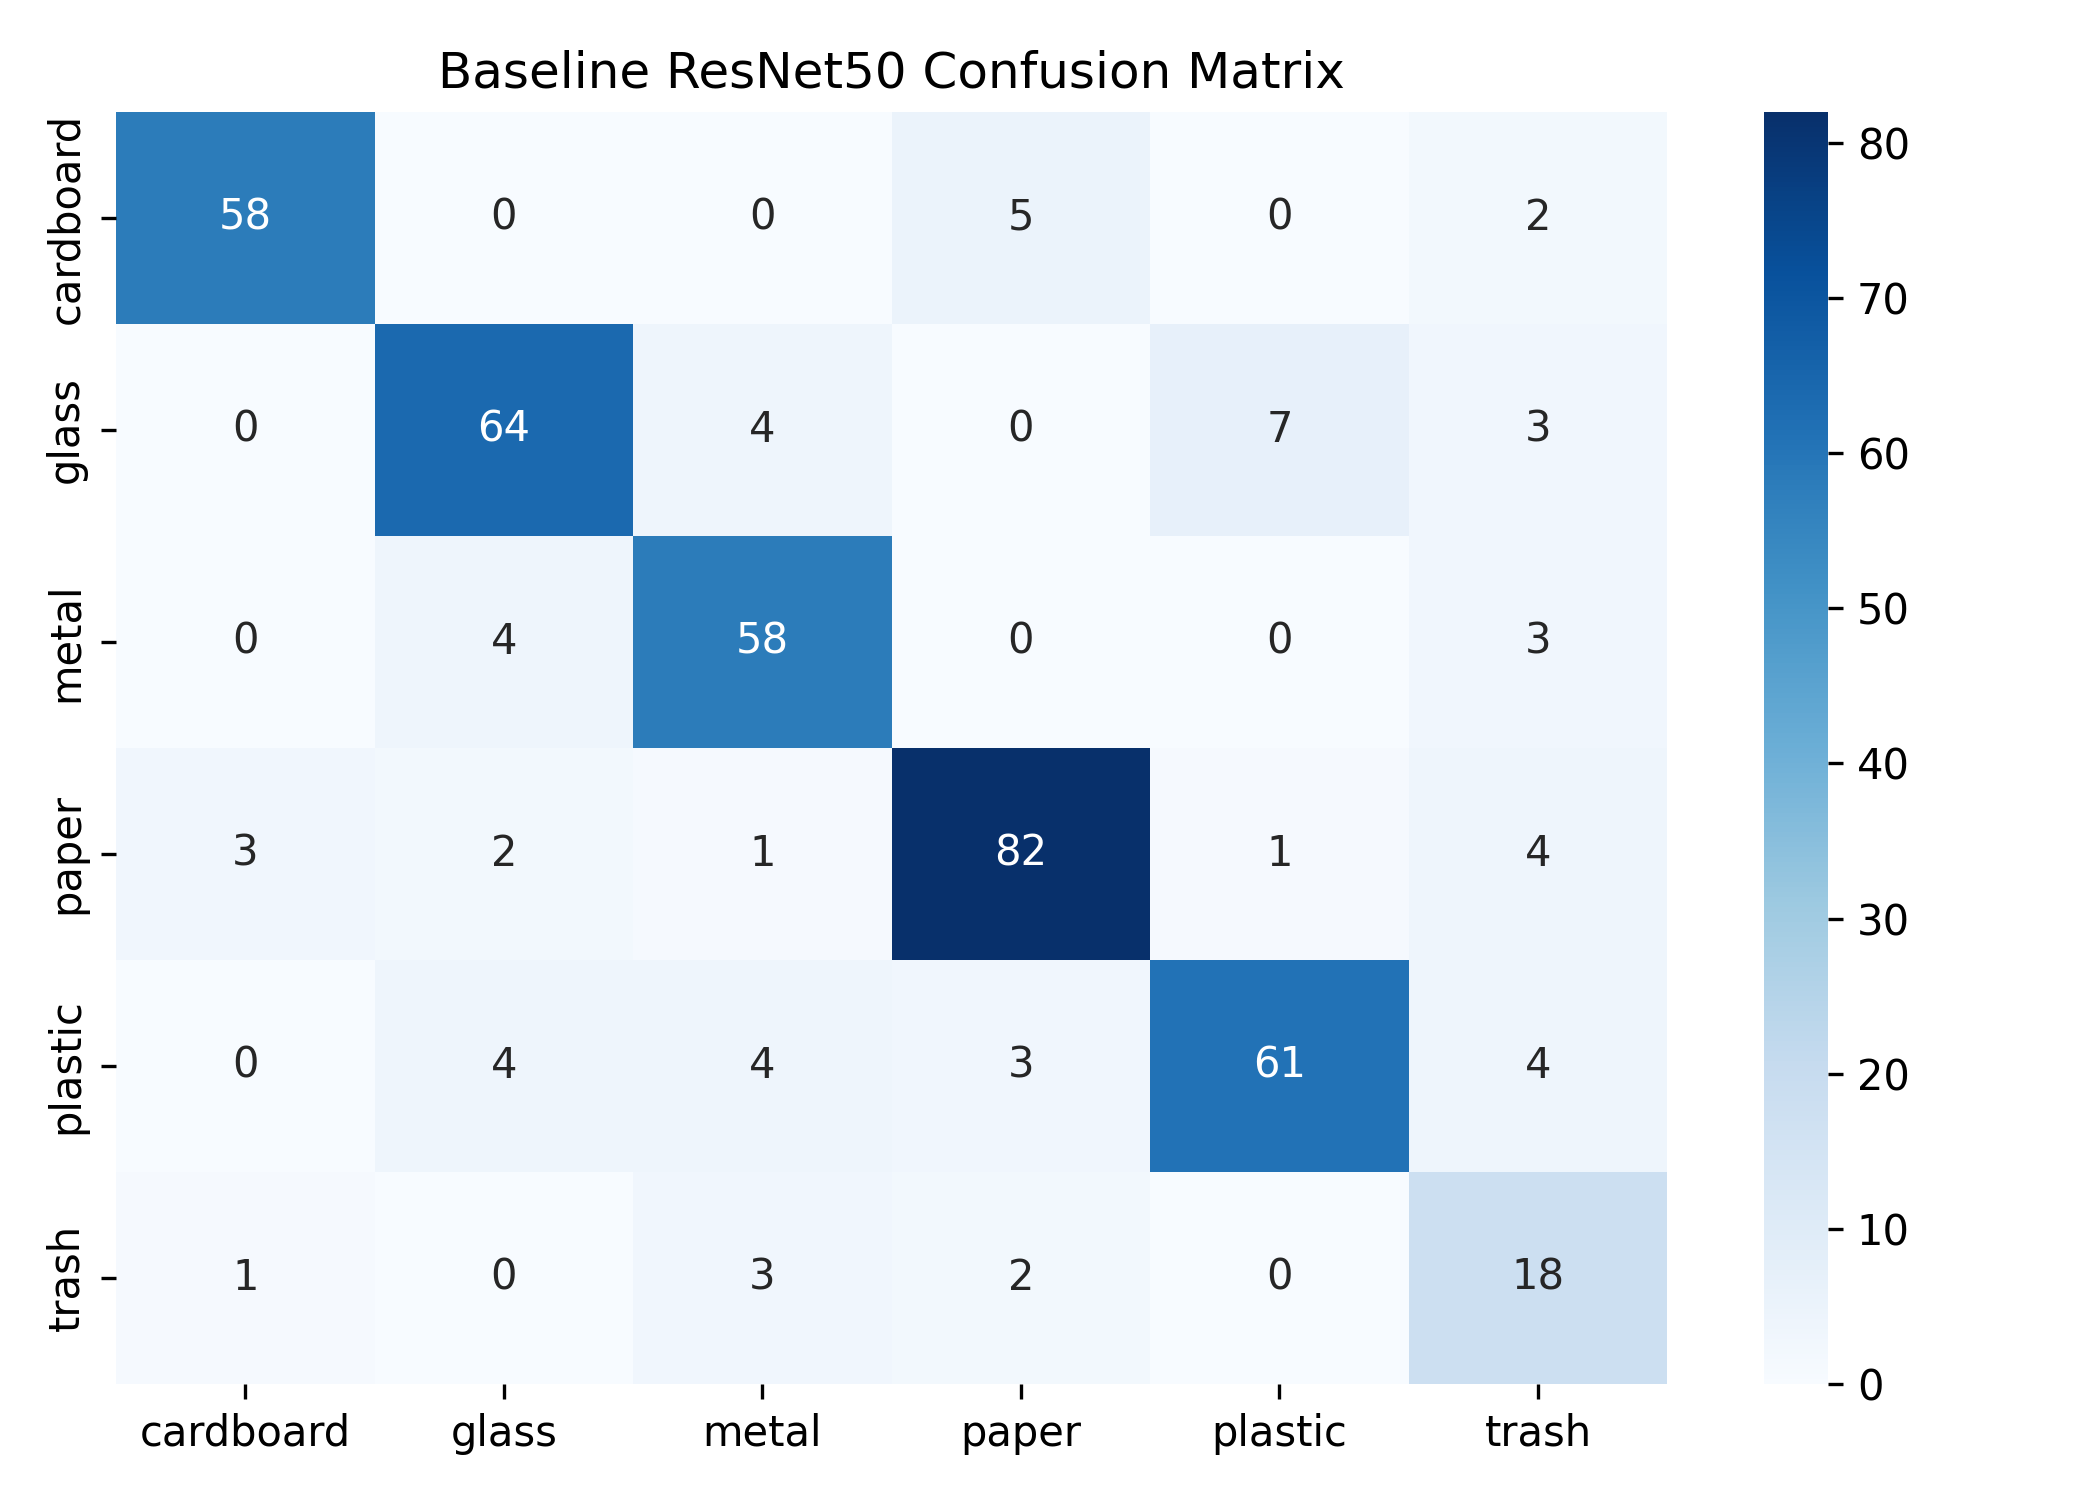
\includegraphics[width=0.78\textwidth]{images/baseline_confusion_matrix.png}
\caption{Baseline confusion matrix generated on the held-out test set.}
\label{fig:baseline-cm}
\end{figure}

\begin{figure}[H]
\centering
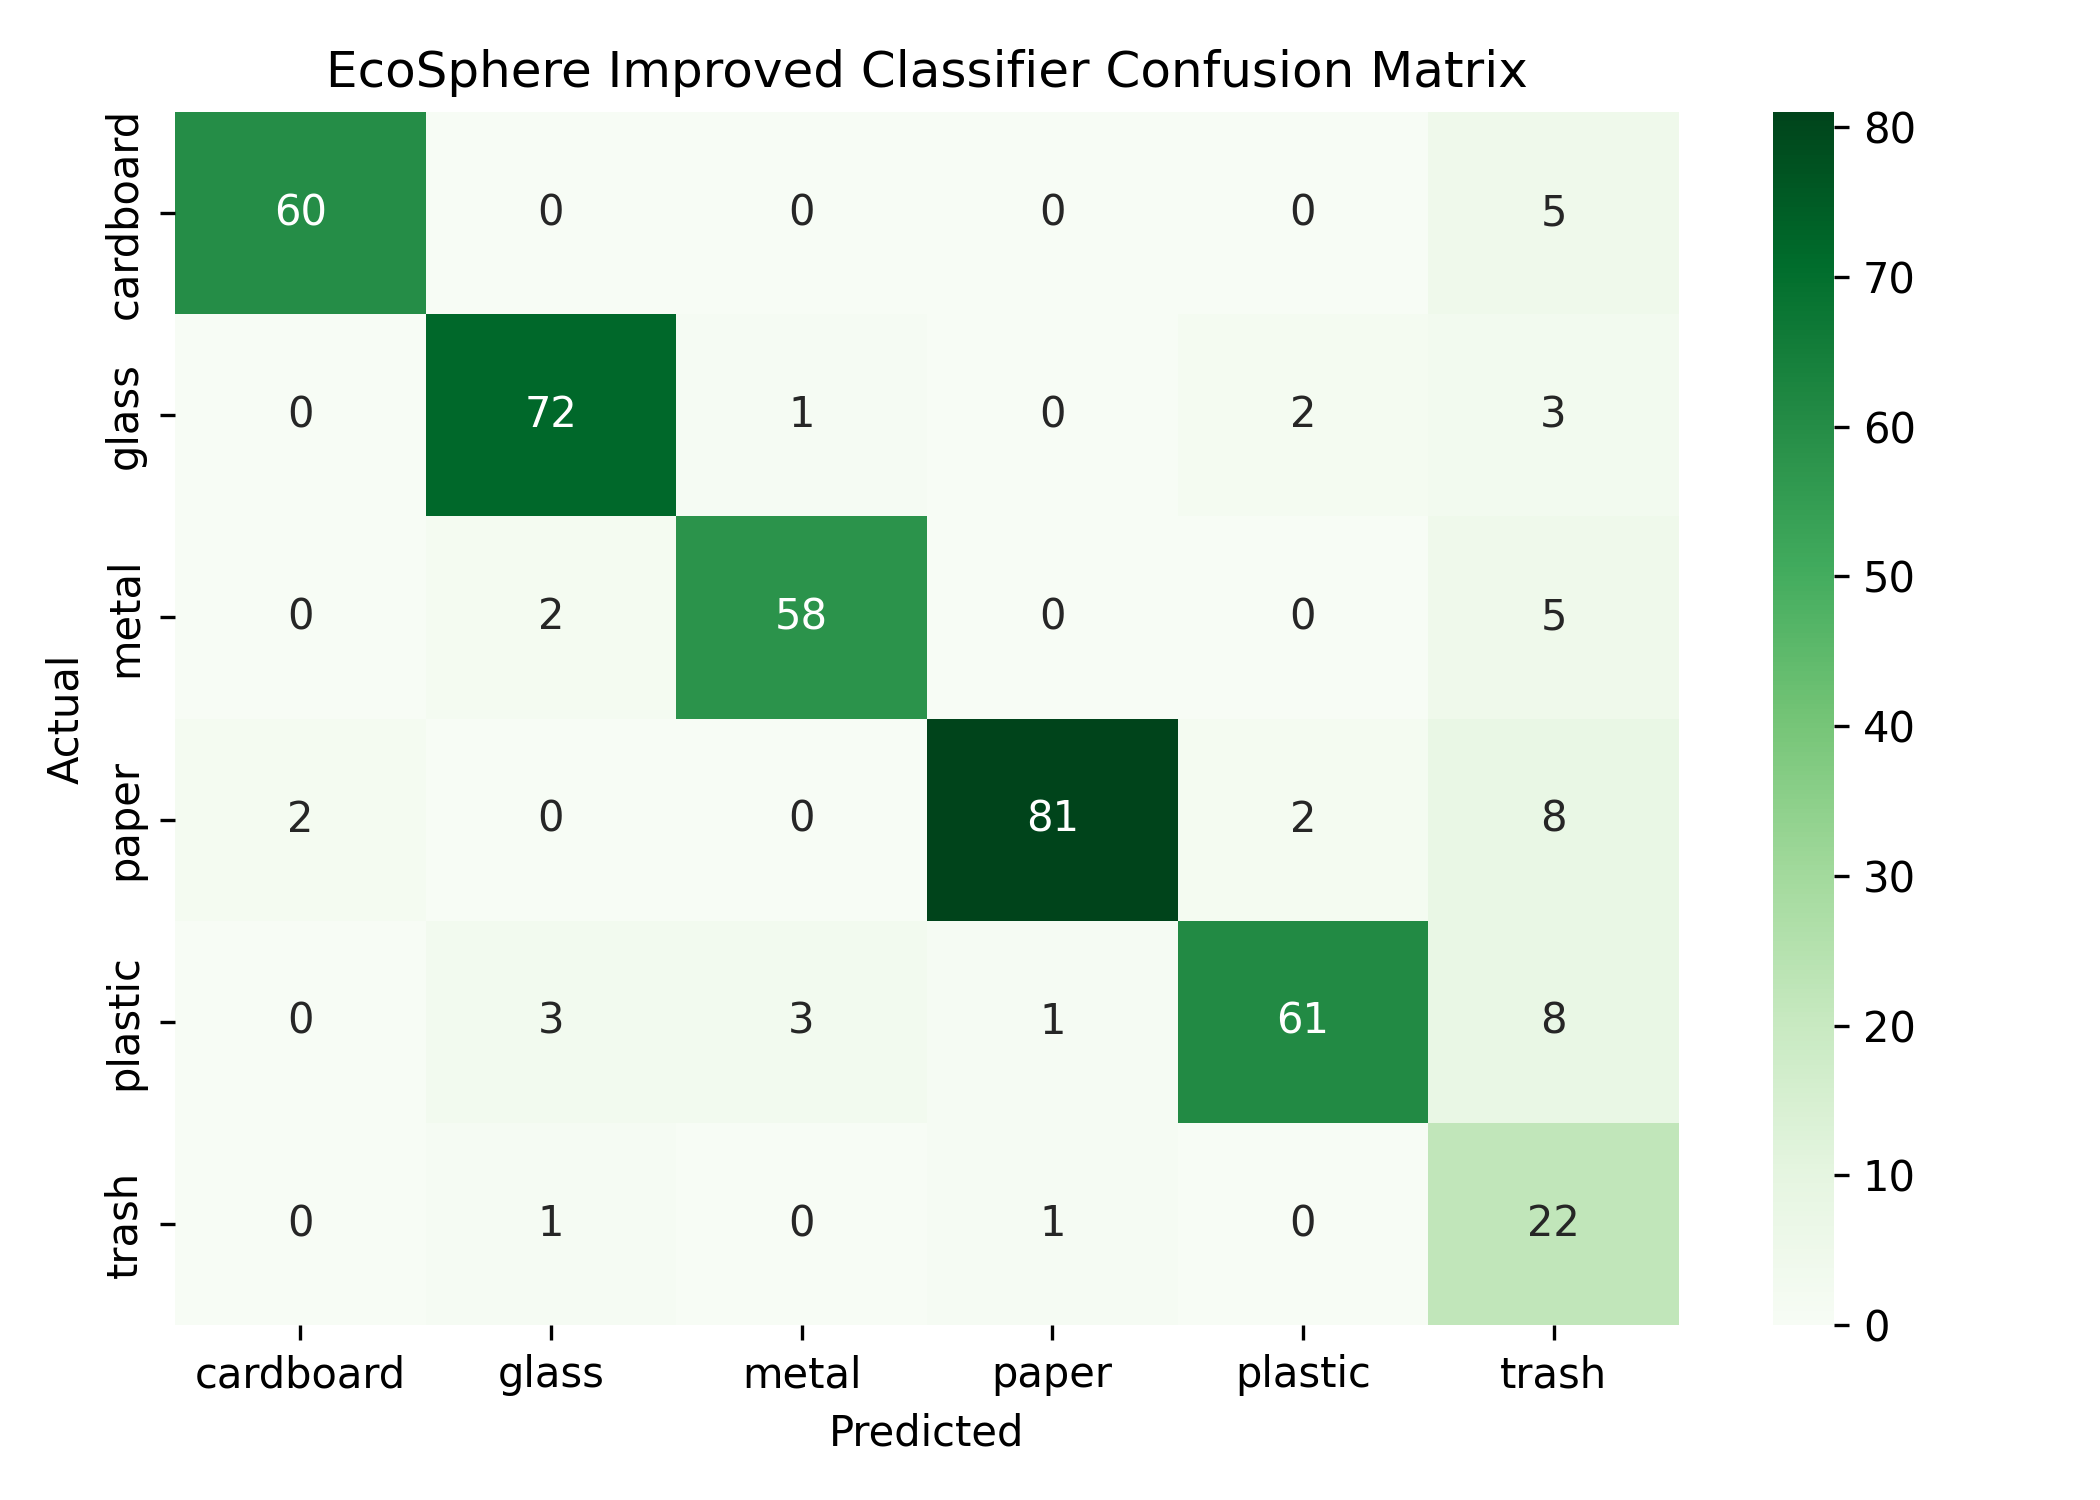
\includegraphics[width=0.78\textwidth]{images/improved_confusion_matrix.png}
\caption{Proposed-model confusion matrix generated on the held-out test set.}
\label{fig:improved-cm}
\end{figure}

\begin{figure}[H]
\centering
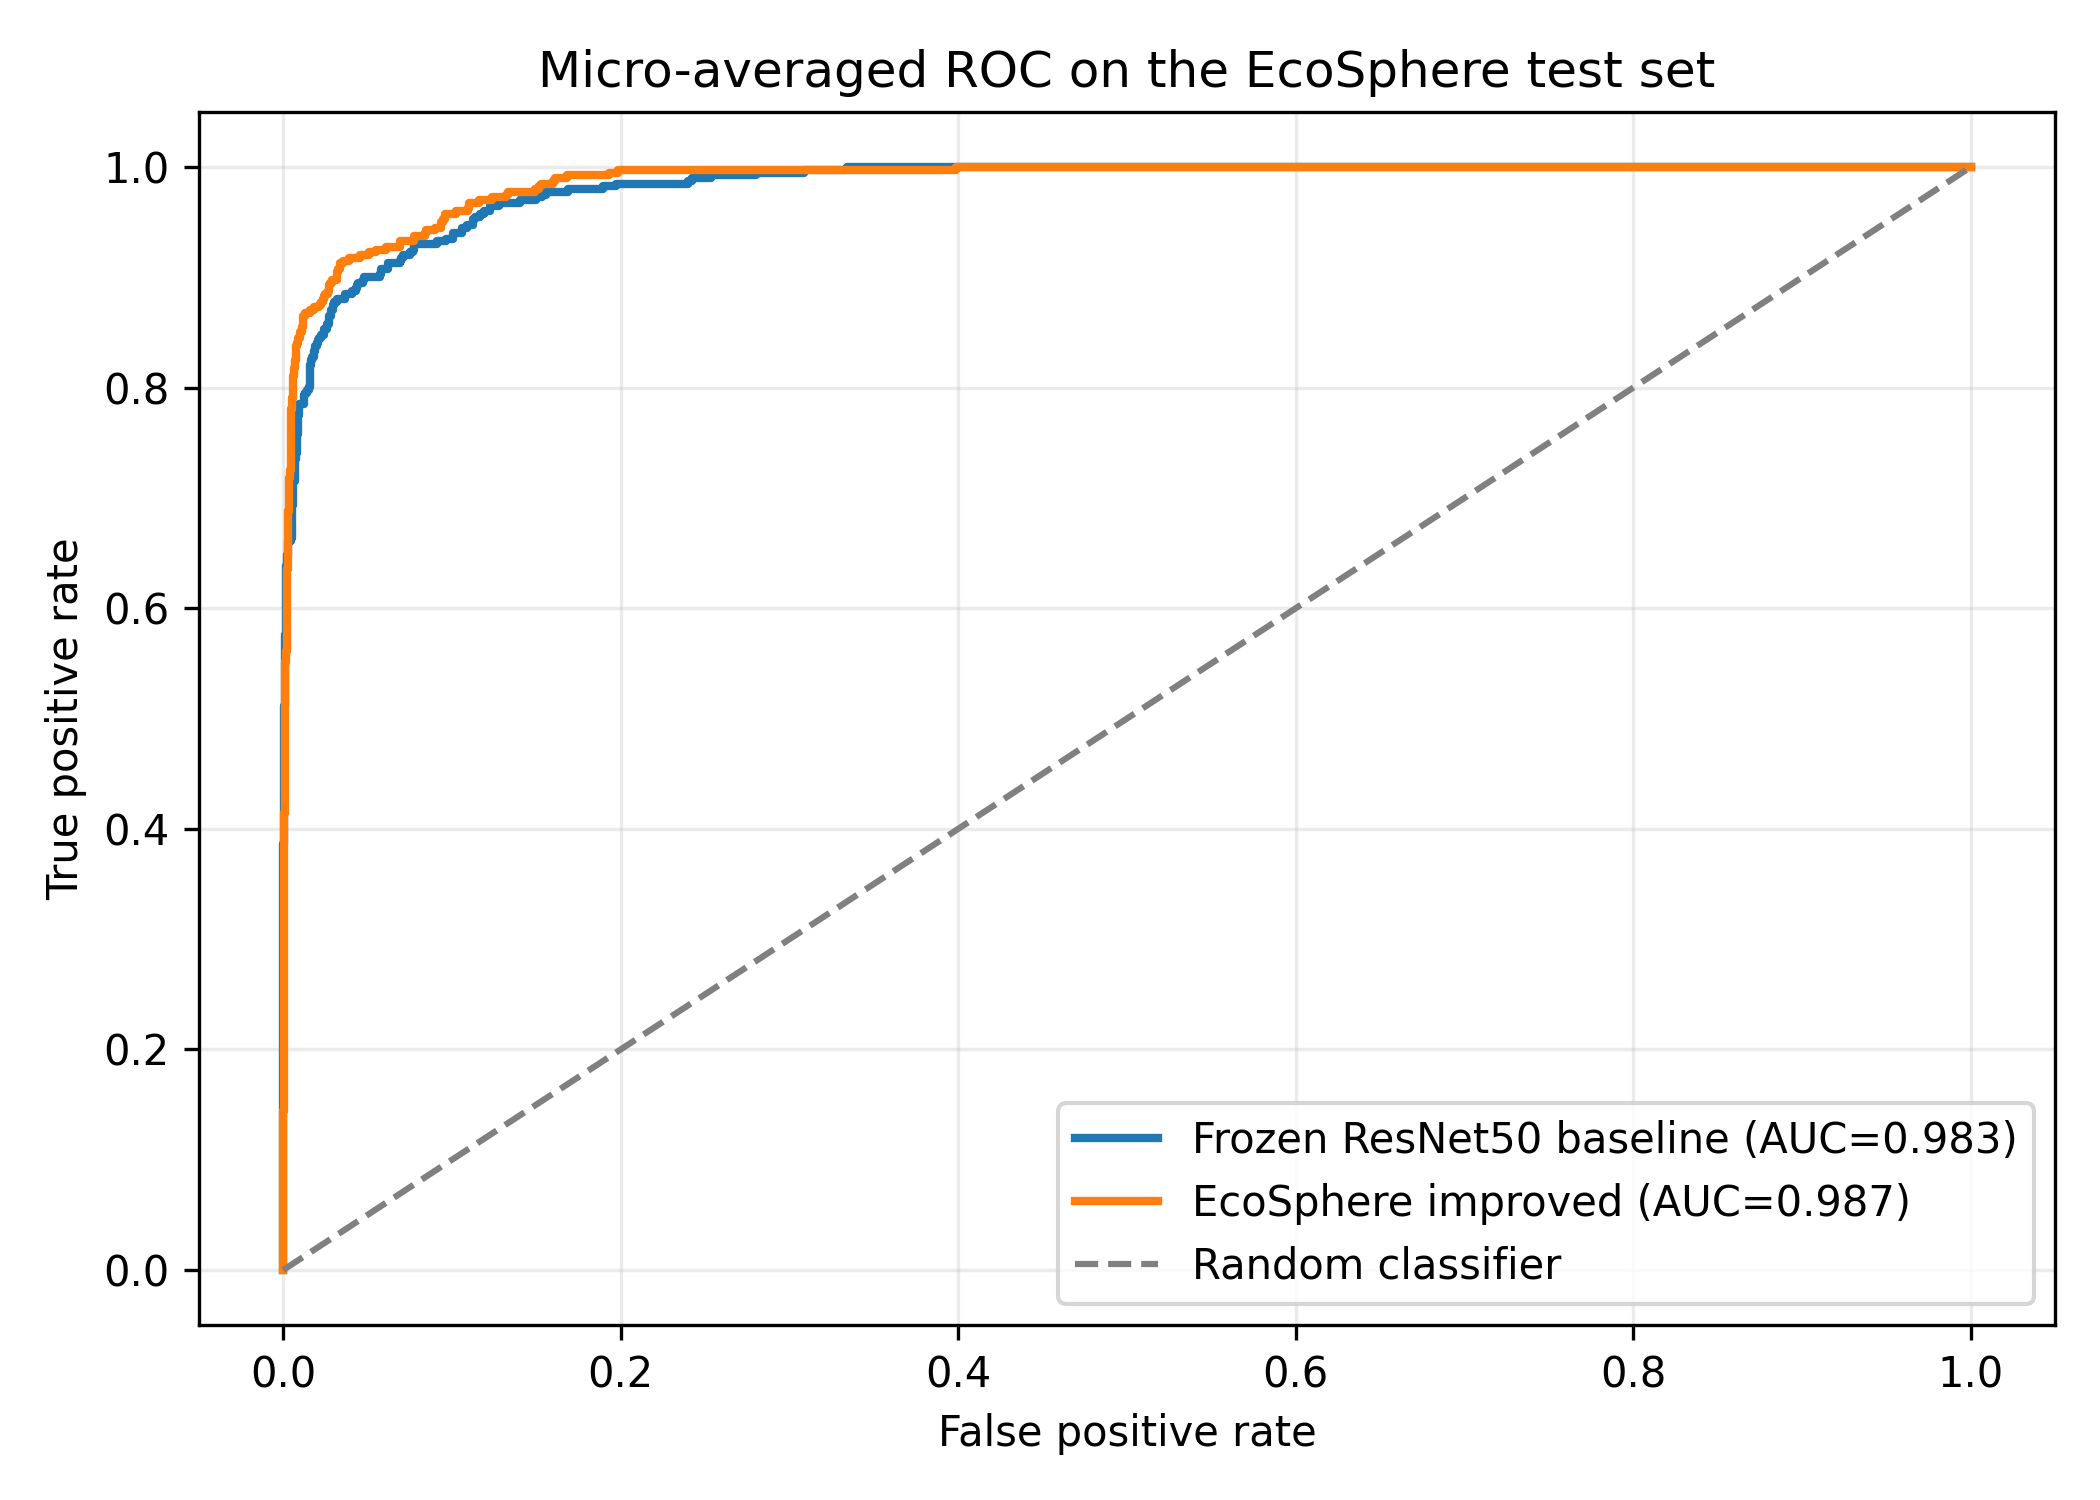
\includegraphics[width=0.78\textwidth]{images/roc_comparison.png}
\caption{Micro-averaged one-vs-rest ROC curves computed from saved probabilities on the common EcoSphere test split.}
\label{fig:roc}
\end{figure}

\section{Discussion}
The proposed classifier head improves accuracy from 85.04\% to 88.28\% under the stated protocol. The improvement is consistent with the intended motivation for focal loss and inverse-frequency weighting: the proposed model substantially increases trash recall. However, the corresponding reduction in trash precision indicates that the method makes more positive trash predictions, including false positives.

The experiment supports the narrow claim that this implemented head performed better than the implemented linear-head baseline on this fixed split. It does not support claims of state-of-the-art performance, generalization to unseen collection sites, superiority to a particular external publication, or production latency. Those claims require additional controlled experiments.

\section{Threats to Validity and Limitations}
\begin{itemize}[leftmargin=*]
  \item The evaluation uses a single fixed train/validation/test split and one reported seed. Repeated seeds or cross-validation are needed to estimate variability.
  \item The dataset is relatively small and may not represent local lighting, camera devices, backgrounds, contamination, or regional waste categories.
  \item The baseline and proposed model use an ImageNet-pretrained backbone, so the comparison isolates the classifier-head and objective changes rather than comparing fully independent architectures.
  \item No inference-latency benchmark was collected in the verified experiment. Latency should be measured on the deployment hardware before making operational claims.
  \item The confusion matrices are visual outputs from the evaluation scripts; exact cell counts should be taken from the evaluation predictions if a numeric matrix is required in a later revision.
\end{itemize}

\section{Reproducibility}
The source scripts are located in the repository under \texttt{research/src/}. The principal commands are:
\begin{verbatim}
python research/src/train_baseline.py
python research/src/train_improved.py
python research/src/generate_metrics.py
python research/src/generate_curves.py
\end{verbatim}
The processed dataset manifest is stored at \texttt{research/dataset/processed/dataset\_manifest.json}. The measured result files are \texttt{research/results/baseline\_results.json} and \texttt{research/results/improved\_results.json}. The manuscript intentionally does not include an external baseline value whose source cannot be verified.

\section{Conclusion}
This paper presents a reproducible comparison for EcoSphere waste image classification. On the verified 378-image test partition, the frozen-ResNet50 linear baseline achieved 85.04\% accuracy and the proposed focal-loss MLP head achieved 88.28\%, an absolute gain of 3.24 percentage points. The proposed model improved minority-class recall but reduced minority-class precision, so future work should evaluate calibration, repeated seeds, external test data, and deployment latency before making broader claims.

\begin{thebibliography}{9}

\bibitem{trashnet}
Gary Thung and Mindy Yang.
\newblock Classification of trash for recyclability status.
\newblock Stanford University CS229 course project report, 2016.
\newblock Dataset repository: \url{https://github.com/garythung/trashnet}.

\bibitem{resnet}
Kaiming He, Xiangyu Zhang, Shaoqing Ren, and Jian Sun.
\newblock Deep residual learning for image recognition.
\newblock In \emph{Proceedings of the IEEE Conference on Computer Vision and Pattern Recognition}, pages 770--778, 2016.

\bibitem{focal}
Tsung-Yi Lin, Priya Goyal, Ross Girshick, Kaiming He, and Piotr Doll\'ar.
\newblock Focal loss for dense object detection.
\newblock In \emph{Proceedings of the IEEE International Conference on Computer Vision}, pages 2980--2988, 2017.

\bibitem{utku2026}
Anil Utku et al.
\newblock From trash to technology: AI-driven waste classification with hybrid CNN-transformer approach for sustainable recycling.
\newblock \emph{Journal of Material Cycles and Waste Management}, 28(1):253--269, 2026.
\newblock \url{https://doi.org/10.1007/s10163-025-02411-4}.

\bibitem{ferrer2025}
Razel M. Ferrer et al.
\newblock Smart waste management: An AI-trainable trash bin for optimized waste segregation.
\newblock \emph{International Journal of Research Publications}, 165(1), 2025.
\newblock \url{https://doi.org/10.47119/IJRP1001651120257475}.

\end{thebibliography}

\end{document}
